\documentclass[12pt]{extarticle}
\usepackage[utf8]{inputenc}
\usepackage{cite}
\usepackage{outlines}
\usepackage{enumitem}
\usepackage{graphicx}
\setenumerate[1]{label=\arabic*}
\setenumerate[2]{label*=.\arabic*}
\setenumerate[3]{label*=.\arabic*}
\setenumerate[4]{label*=.\arabic*}

\begin{document}
\thispagestyle{plain}
\begin{center}
    \Large
    \textbf{Thesis Proposal}
        
    \vspace{0.4cm}
    \large
    Bayesian Hierarchical Spacial Temporal Modeling of Historical Drivers of Global Irrigation Expansion Patterns
        
    \vspace{0.4cm}
    \textbf{Rachel Ledig}
    
    \vspace{0.4cm}
    November 2020
       
\end{center}

\section{Introduction}

Irrigation has the potential to increase productivity of certain crops, function as pest control, and provide food security in semi arid or arid environments where precipitation is low or infrequent (Siebert et al., 2015). These benefits, coupled with increase demand for food, feed and fuel have spurred the expansion of irrigation globally over the past 100 years. According to Siebert et al., (2015) the area equipped for irrigation (AEI) has expanded almost five-fold from 1900 to 2005. At the moment 24 percent of all harvested land is irrigated (Portmann et al., 2010). The trend of irrigation expansion is expected to continue in to the future as more and more demands will be placed on our agricultural systems. Stresses are numerous and global. Increasing populations means more mouths to feed. Rising GDP and urbanization shifts diets toward more animal based products, requiring cultivation of feed stuffs (WHO, n.d.). Agricultural products are no longer only destined for human consumption, biodiesel and bioethanol production have increased the demand for commodity crops (FAO, 2008).  

Increased demand for agricultural products is not the only issue facing the agricultural sector. Water availability, both in terms of supply and demand, will play a crucial role in years to come. On the demand side, global water use has increased six-fold in the past 100 years.  Agriculture remains the largest user with a share of 70 percent of the world's water use, mainly for irrigation (Boretti and Rosa, 2019). Irrigated area harvested is expected to increase as population, therefore food demand increases, especially in developing countries (Neumann et al., 2011). From the supply side, climate change will shift weather patterns and warm the planet, causing a variety of consequences, but most concerning in arid/semi-arid environments, more frequent and longer droughts. Around 20 percent of the world's population lives in arid or semi arid environments (Sivakumar et al., 2005) where precipitation decreases are expected to be 20 percent or more over the coming century (Misra, 2014) further threatening livelihoods and food security in these regions.  	

\section{Aims and Research Questions}

Ultimately, the agricultural system will continue to demand more water while competing with other sectors over decreasing water availability in the coming years. With this pressure farmers will aim to be as efficient as possible by increasing their yields which, in certain areas and under certain conditions, can be done by irrigating their fields. Understanding where, when, and why farmers decide to begin irrigating is important to understand water demands now and in the future. Unfortunately, irrigation expansion is seldom studied, with few studies using statistical modeling techniques to investigate the role that biophysical, economic and political factors play in the spread of irrigation infrastructure in the present. None do so historically. This leads to the first and overarching research question:


\begin{center}
\textbf{Which factors (drivers) have influenced the expansion of irrigation in both time and space over the past 100 years? }

\end{center}
This thesis is aimed at being practical and therefore, both explanatory and predictive models are useful. The ultimate goal is to create models that explain the influence of our drivers on irrigation expansion, the \textbf{best explanatory model}, and models that most accurately predict irrigation fraction given "unknown or new" data, the \textbf{best predictive model}.  These models need not be the same. This gives rise to more research questions:

\begin{center}
\textbf{Which model \emph{explains} historical irrigation patterns best?}

\textbf{Which model \emph{predicts} irrigation expansion best?}

and 
\textbf{What is the difference between these two models?}
\end{center}

By understanding under which conditions irrigation infrastructure is built could be coupled with projections of future climate and economic scenarios, allowing us to get a better idea of scales of agricultural production, land use, and water needs in the coming years. In order to eventually extrapolate to the future, predictive accuracy needs to be addressed. This can be done by separating data into training and testing datasets, model tuning, and error estimation. 


Several other questions smaller questions arise in regard to drivers of expansion which are interesting to investigate. Such as:
\begin{center}
\begin{itemize}
    \item Which has a larger influence on irrigation expansion patterns, biophysical or socio-economic factors?
    \item Do rates of irrigation expansion differ depending on crop type? 
\end{itemize}
\end{center}
Both of these questions have interesting policy implications, should large trends be present in the model and analysis. 

The time series component of this data set also gives rise to some interesting questions.
\begin{center}
\begin{itemize}
    \item Expansion rates of total irrigated area differ temporally, what could be the drivers for this difference? 
    \item Is there a temporal delay in irrigation expansion based on the influence of certain drivers, and if so how much?
\end{itemize}
\end{center}

\section{Literature Review}
In order to get a better grasp of what data, methods and analysis techniques will be needed for this thesis, a light literature review was conducted. Literature can be divided into three sections: studies that aim identify drivers of irrigation expansion from a qualitative perspective, studies that statistically model drivers of irrigation expansion, and studies that use spacial temporal modeling techniques that would be suitable for use in this project. 

\subsection{Irrigation Expansion Drivers}
Studies that explicitly link policies, actions or environmental conditions to irrigation expansion are seldom studied. However, much research exists on irrigation history, policy reform and description of organized collective action to increase irrigation infrastructure. Angelakis et al. (2020) suggest that barriers to irrigation expansion have happened in the past due to investment costs and lack of planing and maintenance, regardless of abundant fresh water resources. Other limitations to expansion over the years have been degradation of irrigation schemes (during the fall of the USSR), competition over available water from other industries (arid and semi-arid regions), and high cost of irrigation technology (developing countries) among other factors (Angelakιs et al., 2020). Wang et al. (2020) discuss the irrigation expansion in China over the past 40 years following shifts in investment, management, and water sources. The authors focus on socio-economic factors only, seldom discussing biophysical features of necessary for expanding irrigation infrastructure, but documenting irrigation increase as a result of policy instruments, water management group schemes, and economic incentives. (Wang et al., 2020). From a qualitative perspective, research suggests that biophysical relationships are not the only drivers of how, when, and why irrigation expands. 

\subsection{Irrigation Modeling}
Neumann et al. (2011) is the most similar study to our proposed thesis topic(s). Neumann et al. attempt to model current irrigation patterns based on biophysical factors (slope, discharge, humidity, ET, evap, pop density, etc) and political factors (democracy, GDP, corruption, political stability) at two different levels, grid cell (5 arc-minute grid cells) and at a country level. However, Neumann's study is only modeling the current irrigation pattern, with no historical perspective. The authors find that the addition of socio-economic information to the model does help improve the explanation the current irrigation pattern, but not only to a small extent. A delay existed, as current patterns are formed from decisions, policies, and economic conditions that occurred years before. Dealing with this issue will also be a focus of this thesis. 

Puy et al. (2020) discusses uncertainties of published projected irrigation expansion patterns by comparing these projections to a simple model that predicts irrigated area as a function of only population size, bounded by available water and land. A simple model was constructed for ease of interpretation, as the main purpose of this study is to discuss uncertainties present in this (seemingly) simple model and investigate how other published projections of irrigation expansion fall within Puy's model's range of uncertainty. Puy's justification for modeling irrigated area as a function of only population size stems from the previous studies showing that population is a variable that encapsulates much more complicated socio-ecological relationships, therefore it is suitable to model irrigation expansion solely based on this variable. 

\subsection{Spacial Temporal Modelling}
The modeling of irrigation expansion is complex, as Neumann and Puy show. However, this thesis attempts elaborate further by not only modelling irrigation patterns in space, but also in time. Literature exists that aims to investigate the complexities of environmental systems using Bayesian hierarchical spacial temporal models (Wikle, 2003; Wikle et al., 1998; Wikle et al., 2001) and, most surprisingly, an area that is really embracing this complex model structure is epidemiology and disease tracking (Bernardinelli et al., 1995; Lawson, 2013). Methods outlined in these studies have helped form the methodology section below. 


\section{Methods}
This is a rough draft of my preliminary variable selection and methods for model formation. I expect this to change over time as I become more well versed in the construction and limitation of these hierarchical models. 
\subsection{Selected Variables}
These variables will be used in model formation. The only exception may be "Discharge" as it only encapsulates surface water. All of these variables available at grid cell level. 
\begin{itemize}
   \item  Provided by Fabian from output of the LPJmL model
   \begin{itemize}
     \item  Distance to the next irrigated grid cell
     \item GDP per capita
     \item Mean and median increase in yield
     \item Latitude and Longitude
    \item Population Density
    \item Discharge - \textbf{Available Surface Water Only}
    \item Crop type
       \end{itemize}
     \end{itemize}
\begin{itemize}
   \item Siebert Data Set
   \begin{itemize}
     \item Converted to Irrigation Fraction
       \end{itemize}
     \end{itemize}   

\subsection{Potential Variables or Data Sets and Limitations}
These are variables that may potentially be included in model formation and analysis. However, majority of these proposed variables are only at country or region level and are not as historical as data from LPJmL. Many are included here as an attempt to capture the influences of socio-economic variables into our model, as from qualitative literature, these factors are important when deciding when to construct irrigation infrastructure. 
\begin{itemize}
   \item  AquaStat data set - Available Water - \textbf{Includes groundwater}
\begin{itemize}
    \item Chosen to encapsulate available water from all sources, including ground water. In many places water supply for irrigation is sourced from groundwater aquifers. 
    \item Data set available from 1956, only in 4-year chunks, only at country level
    \item Used in (Neumann et al., 2011)
    \item Solution: fit model with data only from 56' forward. Total Irrigated Area expanded at a slower rate before this time period. Perhaps there is no need to fit model with data from 1905.
        \end{itemize}   
       \end{itemize}


\begin{itemize}
   \item Political Climate
   \begin{itemize}
   \item Chosen to reflect national governance of irrigation decisions as mentioned in (Neumann et al., 2011) 
     \item Examples of this could be presence of democracy or level of corruption. Exact manifestation of this term could happen in many ways. Neumann does see small improvements to the fit of his model by incorporating this term in.
    \item Historical data sets do exist for this, although “countries” as we know them today have not always had the same boundaries - could complicate analysis. Data sets available in (Neumann et al., 2011).
    \item Solution: Create similar framework to asses political climate as Neumann. OR. Disregard? Perhaps this relationship is manifested within other demographic variables, such as GDP?
       \end{itemize}
     \end{itemize}   

\begin{itemize}
   \item Market Price of Crop or Amount Imported/Exported of Crop
   \begin{itemize}
   \item Listed here to reflect economic incentives to irrigate or not, depending on economic value of particular crop
     \item No complete data set found - And historical data may be difficult to get (MAgPIE data maybe?) 
     \item Solution: Disregard. In (Puy, 2018) and (Puy et al., 2020) the author argues that trade and complex socio-economic relationships are contained within a population or population density variable. So this term may not be needed. Also, the economic incentive to irrigate certain crops more may be seen in the relationship between irrigation fraction per grid cell and crop type present there. 
    \item Will most likely not use for model building and analysis.
       \end{itemize}
     \end{itemize}   
\begin{itemize}
   \item Price of Water
   \begin{itemize}
   \item Again, listed here to reflect economic incentives to irrigate or not, depending on price of water. Which could be a basic issue when deciding to irrigate or not? Could relate to cost benefit analysis of market price of crop - I think too complicated for this thesis?
    \item Solution: Disregard. No good dataset is available and as mentioned in above  
       \end{itemize}
     \end{itemize}  

\begin{itemize}
   \item Technology Costs
   \begin{itemize}
   \item Listed here to reflect upfront economic concerns to irrigate or not, depending on price of local irrigation technology. As mentioned in literature, this can also be a barrier to irrigation expansion in certain places.
     \item No complete data set found - Honestly, this is something that I don't expect to find for current technology, let alone historical prices. 
     \item Solution: Disregard. I only included this as a note. 
       \end{itemize}
     \end{itemize}   

\subsection{Preliminary Data Exploration}
Data exploration is necessary first step for model formation, helping the modeler get a better grasp of the features of her data. This process is very data dependent so, again, these methods are very preliminary. 
\begin{itemize}
   \item Summary Statistics of Variables
   \begin{itemize}
     \item Grid cell level
    \item Country Level
       \end{itemize}
     \end{itemize}   
\begin{itemize}
   \item Plots (+ Temporal Change Detection plots)
   \begin{itemize}
     \item Irrigated Area vs. Country
     \item Irrigated area vs Crop Type
     \item Irrigated Area vs. Temp or humidity 
     \item Irrigated area vs. GDP
       \end{itemize}
     \end{itemize}   
     
\subsection{Model Formation Techniques}
Listed below are some preliminary model formation techniques, taken from resources listed in the bibliography. 

\begin{itemize}
   \item Creation of DAG
   \begin{itemize}
     \item This may be super complex.. 
       \end{itemize}
     \end{itemize}   
\begin{itemize}
    \item Linear Regression Model
\end{itemize}
\begin{itemize}
   \item Bayesian Hierarchical Spacial Temporal Models - Using BRMS package and R
   \begin{itemize}
     \item Investigation of Spacial Auto-correlation - Creation of Co-variance Matrix? (at country and grid level, however, both seem like a lot)
     \item Specification of the Likelihood Function and Distribution
     \item Prior Specification and Regularization for Variables/Parameters
     \item Markov Chain Monte Carlo Simulation
     \item Metropolis Hastings or Gibbs Sampler

       \end{itemize}
     \end{itemize}   

\subsection{Model Tuning and Maintenance}
\begin{itemize}
    \item Trace Plots to ensure efficient sampling of posterior
    \item Monitoring of Effective Sample Size
    \item Dealing with convergence 
\end{itemize}

\subsection{Model Comparison and Cross Validation Techniques}
\begin{itemize}
    \item PSIS, WAIC, AIC, DIC (depending on model and data)
\end{itemize}

\subsection{Explanation vs Prediction}
Here models will be tuned for explanatory or predictive purposes. Methods are still to be selected for this section.


\subsection{Analysis}
Here model outputs will be analyzed and interpreted. Analysis methods will depend on variables selected for models. However, interpretation of coefficients, estimated error, uncertainty, sensitivity analysis, etc will be included here.  



\section{Proposed Outline}
The standard: Abstract,       
Acknowledgments,  
List of Figures, 
List of Tables, 
Glossary.

\begin{outline}[enumerate]

   \1 Introduction
        \2 Nature of the problem of irrigation expansion
        \2 Why is this a modelling irrigation expansion and its drivers an issue? 
        \2 Why is research applicable? 
    
    \1 Literature Review
        \2 Modeling techniques of environmental issues
            \3 Frequentist Techniques Explanation and Usages
            \3 Bayesian Statistical Concepts and Usages
                    \4 Explanation of Bayes Theorem
                    \4 The Prior Distribution
                    \4 The Posterior Distribution
                    \4 Cross Validation Techniques
                    \4 Model Comparison Techniques
        \2 Discussions of potential drivers of irrigation from literature 
            \3 Biophysical Factors
                \4Ex: Available Water
            \3 Demographic Factors
                \4Ex: Population
            \3 External Factors
                \4Ex: Economic issues or policies

    \1 Data and Variables
        \2 Data Sets
            \3 Sibert
                \4 Acquisition
                \4 Description 
                \4 Assumptions 
            \3 LPJmL (same description)
            \3 AquaStat (same description)
        \2 Variables - Description
    \1 Methodology
        \2 Determining of the Likelihood Function
        \2 Determining Priors
        \2 MCMC with Gibbs Sampler
        \2 Model Maintenence
        \2 Model Comparisons
        \2 Model Tuning for Prediction or Explanation
        \2 Analysis Methods
    \1 Models (TBD)
        \2 Linear Regression Model
        \2 Bayesian Model 
            \3 Variables Selected
            \3 Distributions Selected
            \3 Priors Selected
            \3 ...
        \2 Bayesian Hierarchical Model 
        \2 Bayesian Hierarchical Interaction Model
        \2 ...


    \1 Analysis of Models
        \2 Selection of Best Fitting Model
        \2 Selection of Best Predictive Model
        \2 Error Analysis
        \2 Uncertainty and Sensitivity Analysis
        \2 Interpretation of Model Outputs
    \1 Discussion of Models
    \1 Future Research
    \1 Conclusions
    \1 References
    \1 Supplementary Material
\end{outline}

\section{Time Management}
In an effort to improve my time management skills I have attempted to set up a timetable and workflow for this project. The idea behind my thesis process is a series of iterative loops that will allow me to make updates to my models and methods, while contributing to thesis documentation as I go. Below is the iterative work flow I will attempt to follow as I try to answer the research questions. In addition, I have created a timetable which can be found here: https://plan.tomsplanner.com/public/ledigthesisplan. I plan to be finished by the end of April, when Covid is gone and the weather is nicer. 


\begin{center}
   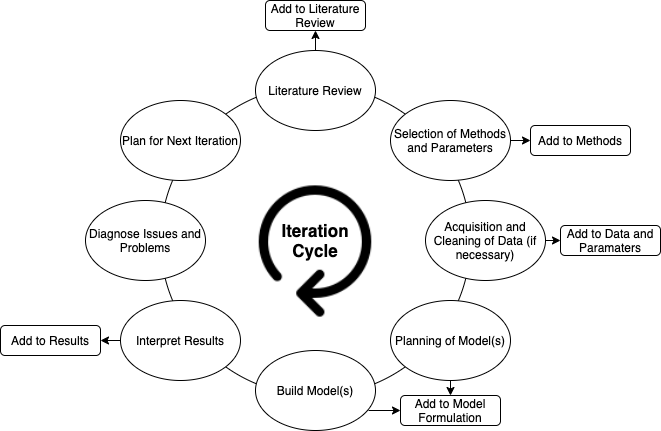
\includegraphics[width=14cm]{Iteration.png}
\end{center}

\section{Bibliography - Notable texts for this thesis}


\textbf{Bernardinelli, L., Clayton, D., Pascutto, C., Montomoli, C., Ghislandi, M., & Songini, M. (1995)}. Bayesian analysis of space—Time variation in disease risk. Statistics in Medicine, 14(21–22), 2433–2443. 
\linebreak https://doi.org/10.1002/sim.4780142112

\textbf{Lawson, A. B. (2013)}. Bayesian Disease Mapping: Hierarchical Modeling in Spatial Epidemiology, Second Edition. CRC Press.

\textbf{Neumann, K., Stehfest, E., Verburg, P. H., Siebert, S., Müller, C., & Veldkamp, T. (2011)}. Exploring global irrigation patterns: A multilevel modelling approach. Agricultural Systems, 104(9), 703–713.

\textbf{Portmann, F. T., Siebert, S., & Döll, P. (2010)}. MIRCA2000—Global monthly irrigated and rainfed crop areas around the year 2000: A new high-resolution data set for agricultural and hydrological modeling. Global Biogeochemical Cycles, 24(1). https://doi.org/10.1029/2008GB003435

\textbf{Puy, A., Lo Piano, S., & Saltelli, A. (2020)}. Current Models Underestimate Future Irrigated Areas. Geophysical Research Letters, 47(8), e2020GL087360. https://doi.org/10.1029/2020GL087360

\textbf{Puy, A. (2018)}. Irrigated areas grow faster than the population. Ecological Applications, 28(6), 1413–1419. https://doi.org/10.1002/eap.1743

\textbf{Shmueli, G. (2010)}. To Explain or to Predict? Statistical Science, 25(3), 289–310. https://doi.org/10.1214/10-STS330

\textbf{Siebert, S., Kummu, M., Porkka, M., Doell, P., Ramankutty, N., & Scanlon, B. (2015)}. A global data set of the extent of irrigated land from 1900 to 2005. Hydrology and Earth System Sciences, 19, 1521–1545. https://doi.org/10.5194/hess-19-1521-2015

\textbf{Wikle, Christopher K. (2003)}. Hierarchical Bayesian Models for Predicting the Spread of Ecological Processes. Ecology, 84(6), 1382–1394. https://doi.org/10.1890/0012-9658(2003)084[1382:HBMFPT]2.0.CO;2

\textbf{Wikle, Christopher K., Berliner, L. M., & Cressie, N. (1998)}. Hierarchical Bayesian space-time models. Environmental and Ecological Statistics, 5(2), 117–154. https://doi.org/10.1023/A:1009662704779

\textbf{Wikle, Christopher K, Milliff, R. F., Nychka, D., & Berliner, L. M. (2001)}. Spatiotemporal Hierarchical Bayesian Modeling Tropical Ocean Surface Winds. Journal of the American Statistical Association, 96(454), 382–397. https://doi.org/10.1198/016214501753168109

\section{References}


\textbf{Angelakιs, A. N., Zaccaria, D., Krasilnikoff, J., Salgot, M., Bazza, M., Roccaro, P., Jimenez, B., Kumar, A., Yinghua, W., Baba, A., Harrison, J. A., Garduno-Jimenez, A., & Fereres, E. (2020)}. Irrigation of World Agricultural Lands: Evolution through the Millennia. Water, 12(5), 1285. https://doi.org/10.3390/w12051285]

\textbf{Boretti, A., & Rosa, L. (2019)}. Reassessing the projections of the World Water Development Report. Npj Clean Water, 2(1), 1–6. \linebreak https://doi.org/10.1038/s41545-019-0039-9

\textbf{FAO. (2008)}. The State of Food and Agriculture 2008. 
\linebreak http://www.fao.org/3/i0100e/i0100e00.htm

\textbf{Misra, A. K. (2014)}. Climate change and challenges of water and food security. International Journal of Sustainable Built Environment, 3(1), 153–165. https://doi.org/10.1016/j.ijsbe.2014.04.006

\textbf{Sivakumar, M., Das, H., & Brunini, O. (2005)}. Impacts of Present and Future Climate Variability and Change on Agriculture and Forestry in the Arid and Semi-Arid Tropics. In Climatic Change (Vol. 70, pp. 31–72). https://doi.org/10.1007/1-4020-4166-7_4

\textbf{Wang, J., Zhu, Y., Sun, T., Huang, J., Zhang, L., Guan, B., & Huang, Q. (2020)}. Forty years of irrigation development and reform in China. Australian Journal of Agricultural and Resource Economics, 64(1), 126–149. https://doi.org/10.1111/1467-8489.12334

\textbf{WHO. (n.d.)}. WHO | 3. Global and regional food consumption patterns and trends. WHO; World Health Organization. Retrieved November 16, 2020, from https://www.who.int/nutrition/topics/3_foodconsumption/en/index4.html

\end{document}
